\documentclass[12pt,a4paper]{article}

\usepackage[utf8]{inputenc}
\usepackage[T1]{fontenc}
\usepackage{geometry}
\usepackage{array}
\usepackage{booktabs}
\usepackage{caption}
\usepackage{enumitem}
\usepackage{fancyhdr}
\usepackage{float}
\usepackage{hyperref}
\usepackage{listings}
\usepackage{longtable}
\usepackage{microtype}
\usepackage{ragged2e}
\usepackage{tabularx}
\usepackage{tikz}
\usetikzlibrary{positioning,arrows.meta}
\usepackage[most]{tcolorbox}
\usepackage{xcolor}
\usepackage{amsmath}
\usepackage{amssymb}
\usepackage{multirow}

\geometry{margin=1in, headheight=15pt}
\hypersetup{
  colorlinks=true,
  linkcolor=blue!70!black,
  urlcolor=blue!70!black,
  citecolor=blue!70!black
}

\definecolor{codegreen}{rgb}{0,0.55,0}
\definecolor{codegray}{rgb}{0.45,0.45,0.45}
\definecolor{codepurple}{rgb}{0.50,0,0.72}
\definecolor{backcolour}{rgb}{0.96,0.96,0.93}
\definecolor{headerblue}{RGB}{30,90,160}
\definecolor{notebox}{RGB}{255,248,220}
\definecolor{infobox}{RGB}{225,240,255}
\definecolor{abbrvbg}{RGB}{240,248,255}
\definecolor{argblue}{RGB}{0,80,160}
\definecolor{fileteal}{RGB}{0,110,110}
\definecolor{symbolpurple}{RGB}{105,45,150}
\definecolor{syntaxorange}{RGB}{190,95,0}
\definecolor{dangerred}{RGB}{170,35,35}
\definecolor{successgreen}{RGB}{20,125,70}
\definecolor{softyellow}{RGB}{255,252,225}
\definecolor{stageblue}{RGB}{210,230,255}
\definecolor{stageyellow}{RGB}{255,250,210}
\definecolor{analogybox}{RGB}{235,245,255}
\definecolor{sidebarbg}{RGB}{248,248,255}

\lstdefinelanguage{LLVM}{
  morekeywords={define,declare,target,triple,source_filename,alloca,load,store,
    call,ret,br,switch,icmp,fcmp,void,i1,i8,i16,i32,i64,float,double,ptr},
  sensitive=true,
  morecomment=[l]{;},
  morestring=[b]"
}

\lstdefinestyle{mystyle}{
  backgroundcolor=\color{backcolour},
  commentstyle=\color{codegreen},
  keywordstyle=\color{magenta},
  numberstyle=\tiny\color{codegray},
  stringstyle=\color{codepurple},
  basicstyle=\ttfamily\footnotesize,
  breakatwhitespace=false,
  breaklines=true,
  captionpos=b,
  keepspaces=true,
  numbers=left,
  numbersep=5pt,
  showspaces=false,
  showstringspaces=false,
  showtabs=false,
  tabsize=2,
  frame=single,
  rulecolor=\color{gray!40}
}
\lstset{style=mystyle}

\newtcolorbox{analogyenv}[1][Think of it like this]{
  colback=analogybox,
  colframe=headerblue!60!black,
  fonttitle=\bfseries,
  title=#1,
  breakable,
  enhanced,
  left=6pt,
  right=6pt,
  top=5pt,
  bottom=5pt
}

\newtcolorbox{noteboxenv}[1][Note]{
  colback=notebox,
  colframe=orange!60!black,
  fonttitle=\bfseries,
  title=#1,
  breakable,
  enhanced
}

\newtcolorbox{infoboxenv}[1][Info]{
  colback=infobox,
  colframe=blue!60!black,
  fonttitle=\bfseries,
  title=#1,
  breakable,
  enhanced
}

\newtcolorbox{sidebarbox}[1][From CPU to Accelerator]{
  colback=sidebarbg,
  colframe=successgreen!70!black,
  fonttitle=\bfseries,
  title=#1,
  breakable,
  enhanced,
  left=6pt,
  right=6pt,
  top=5pt,
  bottom=5pt
}

\newtcolorbox{abbrvbox}{
  colback=abbrvbg,
  colframe=headerblue,
  breakable,
  enhanced,
  left=4pt,
  right=4pt,
  top=4pt,
  bottom=4pt
}

\newtcolorbox{definitionbox}[1][Definition]{
  colback=white,
  colframe=headerblue,
  fonttitle=\bfseries,
  title=#1,
  breakable,
  enhanced,
  left=6pt,
  right=6pt,
  top=5pt,
  bottom=5pt
}

\newtcolorbox{examplebox}[1][Project Example]{
  colback=softyellow,
  colframe=successgreen!70!black,
  fonttitle=\bfseries,
  title=#1,
  breakable,
  enhanced,
  left=6pt,
  right=6pt,
  top=5pt,
  bottom=5pt
}

\pagestyle{fancy}
\fancyhf{}
\fancyhead[L]{\small ONNX to RISC-V Pipeline: ResNet-18 / Gemmini}
\fancyhead[R]{\small\thepage}
\renewcommand{\headrulewidth}{0.4pt}

\newcommand{\file}[1]{\textcolor{fileteal}{\texttt{#1}}}
\newcommand{\filepath}[1]{\begingroup\Urlmuskip=0mu plus 1mu\relax\textcolor{fileteal}{\nolinkurl{#1}}\endgroup}
\newcommand{\cmd}[1]{\textcolor{argblue}{\texttt{\textbf{#1}}}}
\newcommand{\argcmd}[1]{\textcolor{argblue}{\texttt{\textbf{#1}}}}
\newcommand{\syntaxkey}[1]{\textcolor{syntaxorange}{\texttt{\textbf{#1}}}}
\newcommand{\symkey}[1]{\textcolor{symbolpurple}{\texttt{\textbf{#1}}}}
\newcommand{\important}[1]{\textcolor{dangerred}{\textbf{#1}}}
\newcommand{\rowend}{\unskip\hspace{0.5em}\hfill\important{---}}
\newcommand{\okterm}[1]{\textcolor{successgreen}{\textbf{#1}}}
\newcommand{\stageword}[1]{\textcolor{headerblue}{\textbf{#1}}}
\newcommand{\colhead}[1]{\textcolor{headerblue}{\textbf{#1}}}
\newcommand{\abbr}[2]{\textbf{#1} & #2 \\}
\newcolumntype{Y}{>{\RaggedRight\arraybackslash}X}
\newcolumntype{L}[1]{>{\RaggedRight\arraybackslash}p{#1}}

\title{%
  {\Large\bfseries From Neural Network to Hardware Accelerator}\\[6pt]
  {\large Understanding the ONNX to RISC-V + Gemmini Compilation Pipeline}\\[4pt]
  {\normalsize A Practical Guide for Systems Programmers}
}
\author{Technical Documentation}
\date{\today}

\begin{document}

\maketitle

\section*{Plain English Summary}
\addcontentsline{toc}{section}{Plain English Summary}

\subsection*{What This Pipeline Actually Does}

This document describes how we take a neural network model (specifically ResNet-18) and turn it into a program that runs on a RISC-V processor with a Gemmini hardware accelerator. In simple terms:

\begin{itemize}[leftmargin=*]
  \item \textbf{Input:} A ResNet-18 model saved as an ONNX file (about 46 MB of network structure and weights)
  \item \textbf{Output:} A static executable file (about 50 MB) that runs on RISC-V Linux
  \item \textbf{What happens:} The compiler translates the neural network operations into RISC-V CPU code and accelerator library calls
  \item \textbf{How it works:} The model weights become constant data in the executable; the model operations become function calls to a runtime library that talks to the accelerator
\end{itemize}

\subsection*{Why We Need This}

\begin{itemize}[leftmargin=*]
  \item Neural networks are computationally intensive (millions of multiply-add operations)
  \item CPUs alone are too slow for practical inference
  \item Accelerators like Gemmini can perform matrix operations 10-100x faster
  \item We need a way to compile the model to use the accelerator automatically
  \item This pipeline does that: it converts high-level operations into accelerator instructions
\end{itemize}

\subsection*{CPU Programmer's Mental Model}

If you understand CPU programming, you already know most of what's happening here. Here's a quick mapping:

\begin{table}[H]
\centering
\small
\begin{tabularx}{\linewidth}{@{}L{0.28\linewidth}Y@{}}
\toprule
\textbf{Compiler/Accelerator Term} & \textbf{CPU Programming Analogy} \\
\midrule
ONNX Model & A graph of function calls and data dependencies \\
Tensor & A multi-dimensional array with metadata (shape, rank, strides) \\
Weights & Global \texttt{const} arrays initialized with pre-trained values \\
Lowering & Translating high-level code to lower-level code (like Python → C → asm) \\
MLIR Dialect & Different intermediate languages within the compiler toolchain \\
Pass & A transformation that modifies the program representation \\
Memref & A C struct: \texttt{\{void* data; int64\_t* shape; int rank;\}} \\
OMTensor & A standardized C struct for passing tensor data between functions \\
Krnl.call & A function call to a runtime library \\
Runtime Library & Like libc, but for tensor operations \\
ABI & Calling convention and binary interface rules \\
Static Linking & Copying library code directly into your executable (\texttt{gcc -static}) \\
RoCC & A coprocessor interface, similar to SIMD instructions \\
Gemmini & A systolic array accelerator (SIMD on steroids) \\
Scratchpad & On-chip memory managed explicitly (like L2 cache you control) \\
\bottomrule
\end{tabularx}
\caption{Quick translation guide for CPU programmers.}
\end{table}

\begin{sidebarbox}[From CPU to Accelerator]
\small
\textbf{Gemmini is like...} a 16x16 SIMD unit that can do 256 multiplications per cycle, with its own local memory. It's connected to the CPU through custom instructions (RoCC).

\textbf{RoCC (Rocket Custom Coprocessor) is like...} a coprocessor interface similar to how x86 has SIMD instructions, but more flexible. The CPU issues a special instruction, and the accelerator executes it.

\textbf{Systolic array is like...} a 2D pipeline where data flows in a wave, like a conveyor belt of calculations. Each processing element does multiply-add and passes results to its neighbors.

\textbf{Weight-stationary dataflow is like...} keeping the filter weights in the accelerator's local memory and streaming the input data through. Similar to keeping a loop invariant in a register.

\textbf{Scratchpad memory is like...} L2 cache that you manage explicitly. You decide what goes there and when to load/store data.

\textbf{im2col is like...} converting a convolution into a matrix multiply. It's like unrolling a nested loop to use optimized matrix multiply routines.
\end{sidebarbox}

\subsection*{The Big Picture in One Diagram}

\begin{figure}[H]
\centering
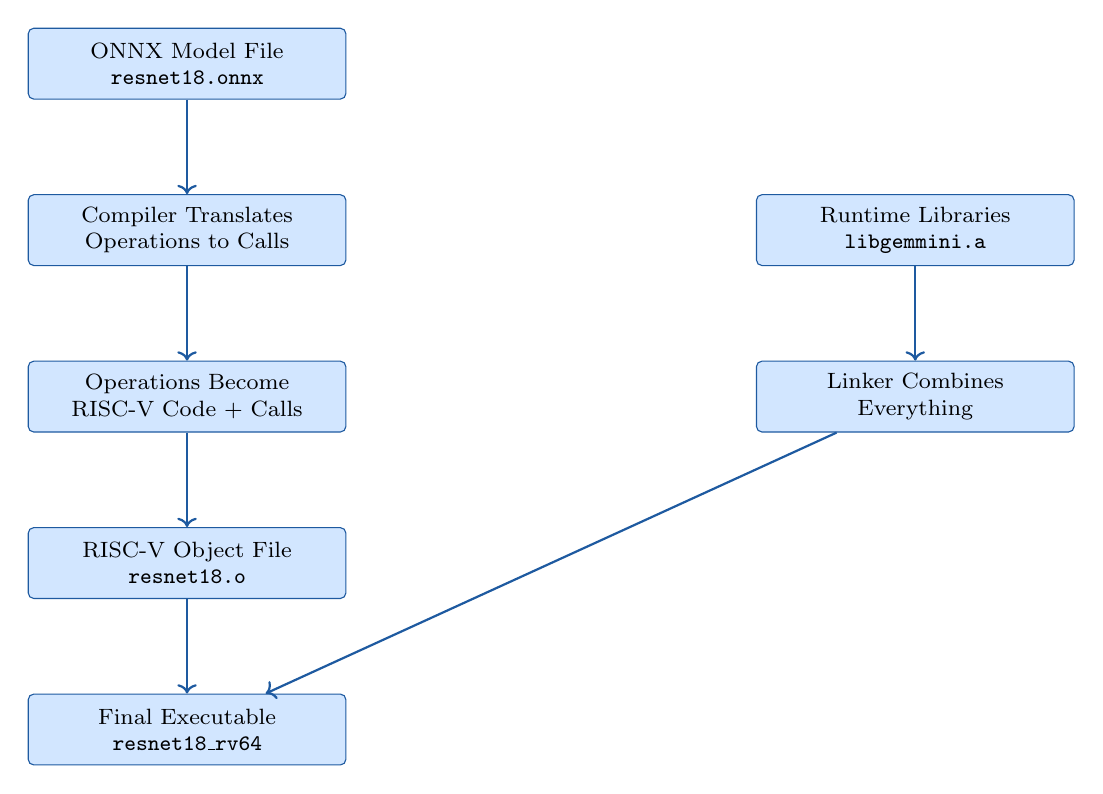
\begin{tikzpicture}[
  node distance=1.2cm,
  stage/.style={rectangle, draw=headerblue, fill=stageblue, rounded corners=2pt,
                text width=3.8cm, align=center, minimum height=0.9cm,
                font=\footnotesize},
  arr/.style={->, thick, draw=headerblue}
]
\node[stage] (s1) {ONNX Model File\\\texttt{resnet18.onnx}};
\node[stage, below=of s1] (s2) {Compiler Translates\\Operations to Calls};
\node[stage, below=of s2] (s3) {Operations Become\\RISC-V Code + Calls};
\node[stage, below=of s3] (s4) {RISC-V Object File\\\texttt{resnet18.o}};
\node[stage, right=of s2, xshift=4cm] (s5) {Runtime Libraries\\\texttt{libgemmini.a}};
\node[stage, below=of s5] (s6) {Linker Combines\\Everything};
\node[stage, below=of s4] (s7) {Final Executable\\\texttt{resnet18\_rv64}};
\draw[arr] (s1) -- (s2);
\draw[arr] (s2) -- (s3);
\draw[arr] (s3) -- (s4);
\draw[arr] (s4) -- (s7);
\draw[arr] (s5) -- (s6);
\draw[arr] (s6) -- (s7);
\end{tikzpicture}
\caption{High-level pipeline flow. The compiler transforms the model into RISC-V code, which is then linked with runtime libraries to produce the final executable.}
\end{figure}

\section*{Key Terms}
\addcontentsline{toc}{section}{Key Terms}

\noindent
\textbf{ONNX-MLIR:} The compiler that reads ONNX models and generates MLIR
\textbf{MLIR:} Multi-Level Intermediate Representation - a compiler framework with multiple languages
\textbf{LLVM IR:} Low-level virtual machine intermediate representation (like assembly with unlimited registers)
\textbf{RISC-V:} Open instruction set architecture for CPUs
\textbf{Gemmini:} Hardware accelerator for matrix operations
\textbf{RoCC:} Rocket Custom Coprocessor - interface for accelerators
\textbf{ResNet-18:} A neural network architecture with 18 layers
\textbf{Static Linking:} Combining all code into one executable (no shared libraries at runtime)
\textbf{OMTensor:} Runtime data structure for passing tensors between compiler-generated code and runtime libraries

\vspace{0.8em}

\tableofcontents
\newpage

\section{Introduction: What We're Building}

This document describes the complete process of taking a ResNet-18 neural network model (saved as an ONNX file) and turning it into a RISC-V executable that uses the Gemmini hardware accelerator. The final output is a self-contained static executable that can run on RISC-V hardware with Gemmini support.

\begin{examplebox}[What's in the Final Executable]
The executable \texttt{resnet18\_rv64} (about 50 MB) contains:
\begin{itemize}
  \item The compiled ResNet-18 model code (which layer to run, in what order)
  \item All model weights (converted to constant data in \texttt{.rodata})
  \item The Gemmini runtime library (code that talks to the accelerator)
  \item The ONNX-MLIR runtime library (tensor management)
  \item System libraries (math functions, memory management)
  \item A test harness (the \texttt{main()} function)
\end{itemize}
\end{examplebox}

\subsection{What Problem Does This Solve?}

\begin{itemize}[leftmargin=*]
  \item \textbf{Neural networks are slow on CPUs:} Each inference involves millions of multiply-add operations. A typical CNN layer might need 100 million operations for a single image.
  \item \textbf{Hardware accelerators exist but need special code:} Gemmini is a systolic array that can do many multiplications in parallel, but you need to tell it what to do through custom instructions.
  \item \textbf{We need automation:} Manually rewriting neural networks to use accelerators is impossible for large models. We need a compiler to do it automatically.
  \item \textbf{This pipeline provides the automation:} It takes the high-level model description and generates executable code that uses the accelerator efficiently.
\end{itemize}

\begin{analogyenv}[Think of it like compiling C]
When you compile C code:
\begin{enumerate}
  \item You write high-level code (\texttt{for} loops, function calls)
  \item The compiler translates it to assembly instructions
  \item The assembler creates object files
  \item The linker combines them into an executable
\end{enumerate}

This pipeline does the same thing, but for neural networks:
\begin{enumerate}
  \item The model is described as operations (convolution, matrix multiply, activation)
  \item The compiler translates these to function calls (to the accelerator runtime)
  \item The runtime library implements those functions using hardware instructions
  \item Everything is linked into one executable
\end{enumerate}
\end{analogyenv}

\subsection{Why Two Compilers?}

You might wonder: why can't we just use one compiler? The answer is division of labor:

\begin{table}[H]
\centering
\small
\begin{tabularx}{\linewidth}{@{}L{0.30\linewidth}L{0.35\linewidth}Y@{}}
\toprule
\textbf{Compiler} & \textbf{What It's Good At} & \textbf{What It Produces} \\
\midrule
ONNX-MLIR (LLVM-based) & Understanding neural network structure, tensor shapes, and operations & RISC-V object code for the model itself \\
GCC (GNU Compiler Collection) & Compiling C/C++ runtime libraries, system code & Runtime libraries (OMTensor, Gemmini runtime) \\
\bottomrule
\end{tabularx}
\end{table}

The two compilers meet in the middle through the ABI (Application Binary Interface):
- ONNX-MLIR generates code that calls functions like \texttt{om\_gemmini\_conv\_f32()}
- GCC compiles the implementation of those functions
- The linker connects the calls to the implementations

\begin{analogyenv}[Think of it like this]
Imagine you're writing a program that uses the \texttt{sin()} function:
\begin{enumerate}
  \item You write code that calls \texttt{sin(x)}
  \item Your compiler generates a call to an external symbol
  \item The linker connects that call to the math library (\texttt{-lm})
  \item The math library is pre-compiled and contains the actual implementation
\end{enumerate}

The same thing happens here:
\begin{enumerate}
  \item The compiled model calls \texttt{om\_gemmini\_conv\_f32(...)}
  \item The linker connects that call to the Gemmini runtime library
  \item The Gemmini runtime library contains the actual accelerator implementation
\end{enumerate}
\end{analogyenv}

\subsection{What's in This Document}

This document walks through the entire pipeline step by step. For each stage, you'll learn:
\begin{itemize}[leftmargin=*]
  \item \textbf{What problem it solves} - why we can't skip this stage
  \item \textbf{What it does in plain English} - the core transformation
  \item \textbf{CPU programming analogy} - how this is like something you already know
  \item \textbf{Before and after examples} - what the code looks like at each stage
  \item \textbf{What goes wrong if we skip it} - the consequences of omission
\end{itemize}

\section{The Runtime Directory: Understanding the Bridge}

Before diving into the pipeline, let's look at the runtime directory. This is where the bridge between the compiled model and the accelerator lives.

\begin{infoboxenv}[What's in the Runtime Directory]
The runtime directory (\texttt{src/Accelerators/Gemmini/Runtime/}) contains:
\begin{itemize}
  \item \textbf{OMRuntimeGemmini.hpp/cpp:} The main implementation of accelerator operations
  \item \textbf{gemmini-hardware-abi/:} Bundled Gemmini hardware headers
  \item \textbf{CMakeLists.txt:} Build configuration
  \item \textbf{FILES\_EXPLAINED.md:} Documentation
\end{itemize}

This directory is the translator between compiler-generated calls and actual accelerator instructions.
\end{infoboxenv}

\begin{sidebarbox}[Understanding the Runtime Files]
Let's map these to CPU concepts:
\begin{itemize}
  \item \texttt{OMRuntimeGemmini.hpp} is like a header file that declares functions you'll call
  \item \texttt{OMRuntimeGemmini.cpp} is like the implementation of those functions
  \item \texttt{gemmini-hardware-abi/} is like the CPU's instruction set manual (but for the accelerator)
  \item The compiled \texttt{libgemmini\_f32\_rv64.a} is like a static library you link with
\end{itemize}
\end{sidebarbox}

\subsection{What Each Runtime File Does}

\begin{table}[H]
\centering
\small
\begin{tabularx}{\linewidth}{@{}L{0.30\linewidth}L{0.35\linewidth}Y@{}}
\toprule
\textbf{File} & \textbf{CPU Programmer's Understanding} & \textbf{What It Actually Does} \\
\midrule
\texttt{OMRuntimeGemmini.hpp} & Header file declaring accelerator functions & Declares \texttt{om\_gemmini\_conv\_f32}, \texttt{om\_gemmini\_matmul}, etc. with \texttt{extern "C"} \\
\texttt{OMRuntimeGemmini.cpp} & Implementation of those functions & Implements convolution, matrix multiply, pooling, activation functions \\
\texttt{gemmini-hardware-abi/} & CPU instruction set documentation & Defines the low-level interface to Gemmini (RoCC instructions, register layout) \\
\texttt{CMakeLists.txt} & Makefile alternative & Controls compilation, finds headers, sets flags \\
\bottomrule
\end{tabularx}
\end{table}

\begin{analogyenv}[Think of it like hardware drivers]
The Gemmini runtime is like a device driver for a GPU or a custom accelerator:
\begin{itemize}
  \item \texttt{OMRuntimeGemmini.cpp} is the driver implementation
  \item It translates high-level operations (like "do a convolution") into low-level hardware commands
  \item \texttt{gemmini-hardware-abi/} is the hardware specification
  \item The driver knows how to configure the hardware, move data, and execute operations
\end{itemize}

When your compiled model calls \texttt{om\_gemmini\_conv\_f32()}, it's like calling \texttt{write()} on a device file. The runtime driver translates it into the actual hardware commands.
\end{analogyenv}

\subsection{The Runtime Flow in Practice}

\begin{figure}[H]
\centering
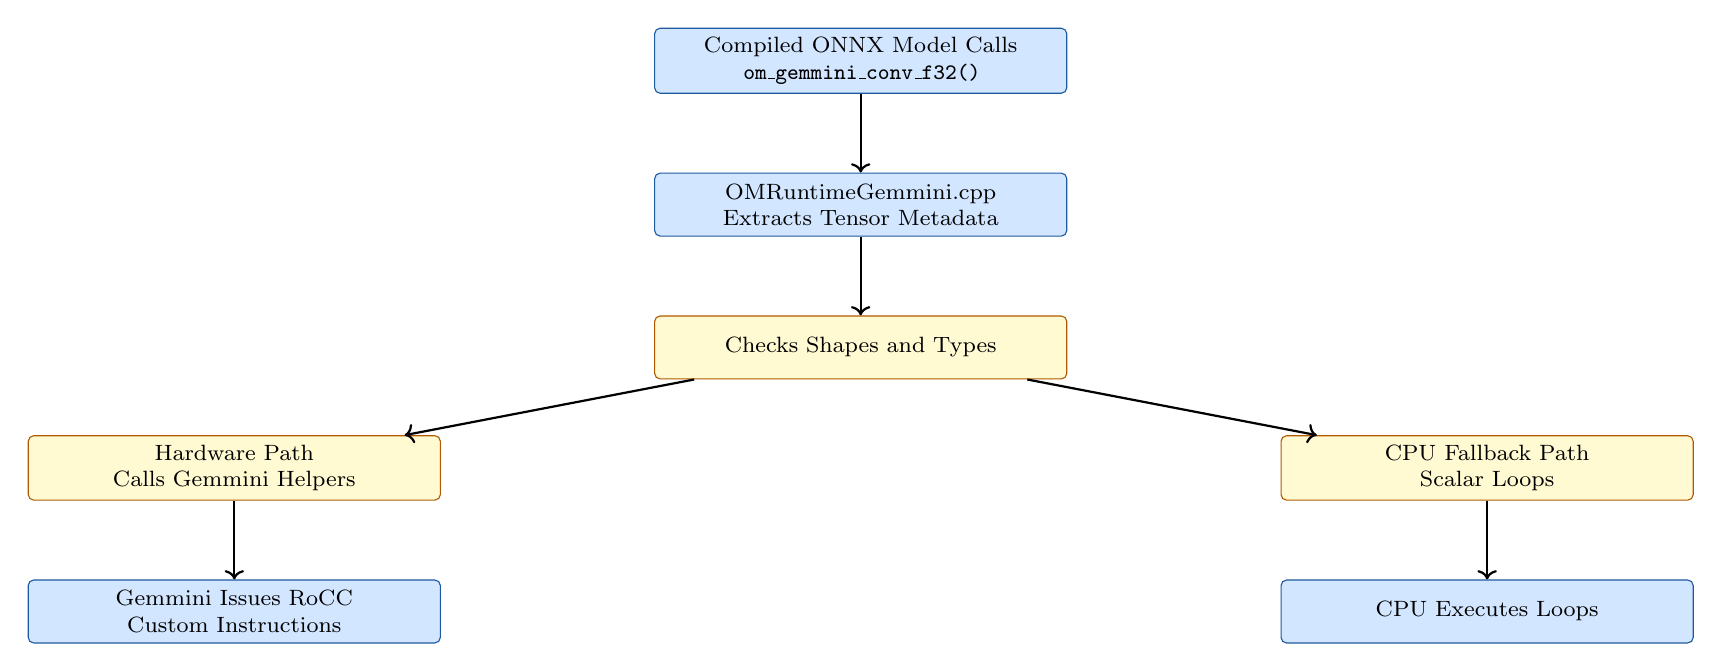
\begin{tikzpicture}[
  node distance=1cm,
  flow/.style={rectangle, draw=headerblue, fill=stageblue, rounded corners=2pt,
               text width=5.0cm, align=center, minimum height=0.8cm,
               font=\footnotesize},
  hw/.style={rectangle, draw=orange!70!black, fill=stageyellow, rounded corners=2pt,
             text width=5.0cm, align=center, minimum height=0.8cm,
             font=\footnotesize},
  arr/.style={->, thick}
]
\node[flow] (model) {Compiled ONNX Model Calls\\\texttt{om\_gemmini\_conv\_f32()}};
\node[flow, below=of model] (runtime) {OMRuntimeGemmini.cpp\\Extracts Tensor Metadata};
\node[hw, below=of runtime] (dispatch) {Checks Shapes and Types};
\node[hw, below left=of dispatch, xshift=-2cm] (hardware) {Hardware Path\\Calls Gemmini Helpers};
\node[hw, below right=of dispatch, xshift=2cm] (cpu) {CPU Fallback Path\\Scalar Loops};
\node[flow, below=of hardware] (rocc) {Gemmini Issues RoCC\\Custom Instructions};
\node[flow, below=of cpu] (scalar) {CPU Executes Loops};
\draw[arr] (model) -- (runtime);
\draw[arr] (runtime) -- (dispatch);
\draw[arr] (dispatch) -- (hardware);
\draw[arr] (dispatch) -- (cpu);
\draw[arr] (hardware) -- (rocc);
\draw[arr] (cpu) -- (scalar);
\end{tikzpicture}
\caption{Runtime execution flow. The runtime decides whether to use the accelerator or fall back to CPU.}
\end{figure}

\subsection{Understanding the Gemmini ABI Headers}

The \texttt{gemmini-hardware-abi/} directory bundles the headers needed to talk to Gemmini. Here's what each file does:

\begin{table}[H]
\centering
\small
\begin{tabularx}{\linewidth}{@{}L{0.30\linewidth}L{0.35\linewidth}Y@{}}
\toprule
\textbf{Header File} & \textbf{CPU Programmer's Understanding} & \textbf{What It Defines} \\
\midrule
\texttt{gemmini.h} & Main API header & \texttt{tiled\_matmul\_auto}, \texttt{tiled\_conv\_auto}, configuration functions \\
\texttt{gemmini\_params.h} & CPU feature flags & Array size (16), data types (\texttt{int8\_t}, \texttt{int32\_t}), scratchpad sizes \\
\texttt{gemmini\_nn.h} & Neural network helper functions & High-level conv/pooling helpers, parameter structs \\
\texttt{gemmini\_counter.h} & Performance counters & Cycle counters, DMA counters, etc. \\
\texttt{xcustom.h} & Custom instruction macros & Macros that emit actual RISC-V custom instructions \\
\bottomrule
\end{tabularx}
\end{table}

\section{Pipeline Overview: The Nine Stages}

Here's the complete pipeline at a glance. The diagram below shows what each stage does and what files it produces.

\begin{figure}[H]
\centering
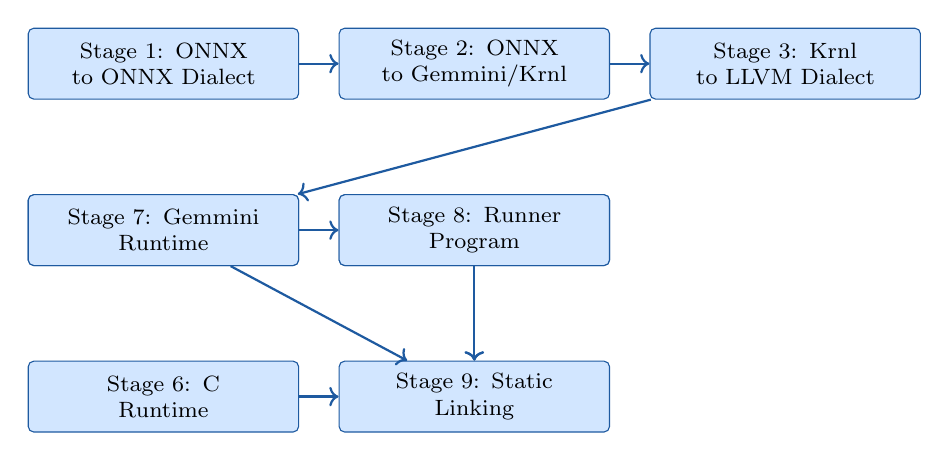
\begin{tikzpicture}[
  node distance=1.2cm and 0.5cm,
  stage/.style={rectangle, draw=headerblue, fill=stageblue, rounded corners=2pt,
                text width=3.2cm, align=center, minimum height=0.9cm,
                font=\footnotesize},
  arr/.style={->, thick, draw=headerblue}
]
\node[stage] (s1) {Stage 1: ONNX\\to ONNX Dialect};
\node[stage, right=of s1] (s2) {Stage 2: ONNX\\to Gemmini/Krnl};
\node[stage, right=of s2] (s3) {Stage 3: Krnl\\to LLVM Dialect};
\node[stage, below=of s1] (s4) {Stage 4: Dialect\\to LLVM IR};
\node[stage, right=of s4] (s5) {Stage 5: LLVM IR\\to Object File};
\node[stage, below=of s5] (s9) {Stage 9: Static\\Linking};
\node[stage, left=of s9] (s6) {Stage 6: C\\Runtime};
\node[stage, above=of s6] (s7) {Stage 7: Gemmini\\Runtime};
\node[stage, right=of s7] (s8) {Stage 8: Runner\\Program};
\draw[arr] (s1) -- (s2);
\draw[arr] (s2) -- (s3);
\draw[arr] (s3) -- (s4);
\draw[arr] (s4) -- (s5);
\draw[arr] (s5) -- (s9);
\draw[arr] (s6) -- (s9);
\draw[arr] (s7) -- (s9);
\draw[arr] (s8) -- (s9);
\end{tikzpicture}
\caption{The nine stages of the compilation pipeline. Stages 1-5 produce the model object; Stages 6-8 produce support libraries; Stage 9 links everything together.}
\end{figure}

\begin{table}[H]
\centering
\small
\begin{tabularx}{\linewidth}{@{}L{0.07\linewidth}L{0.25\linewidth}L{0.25\linewidth}Y@{}}
\toprule
\textbf{Stage} & \textbf{Input} & \textbf{Output} & \textbf{What Happens} \\
\midrule
1 & ONNX model & ONNX dialect MLIR & Parse the model into compiler's internal representation \\
2 & ONNX dialect & Krnl/Gemmini MLIR & Replace operations with runtime calls where possible \\
3 & Krnl/Gemmini & LLVM dialect MLIR & Convert to LLVM's internal representation \\
4 & LLVM dialect & LLVM IR text & Export as standard LLVM assembly \\
5 & LLVM IR & RISC-V object file & Generate RISC-V machine code \\
6 & C runtime sources & Static archive & Build ONNX-MLIR tensor management library \\
7 & C++ runtime sources & Static archive & Build Gemmini accelerator library \\
8 & Runner C source & Object file & Build test harness with \texttt{main()} \\
9 & Objects + archives & Static executable & Link everything into one ELF file \\
\bottomrule
\end{tabularx}
\end{table}

\section{Stage-by-Stage Breakdown}

\subsection{Stage 1: ONNX to ONNX Dialect}

\begin{analogyenv}[Think of it like reading a header file]
Stage 1 is like the compiler reading a \texttt{.h} file. It parses the ONNX file and builds an internal representation. The compiler doesn't generate code yet - it just understands what the model looks like.
\end{analogyenv}

\subsubsection{What Problem Does This Solve?}
The ONNX file is a binary protobuf format. We need to convert it into a format that the compiler can manipulate. This stage parses the binary and creates an MLIR representation.

\subsubsection{What It Does}
\begin{itemize}
  \item Reads the ONNX protobuf file
  \item Parses the graph structure (which operations, in what order)
  \item Imports tensor initializers (weights) as constants
  \item Creates MLIR operations like \texttt{onnx.Conv}, \texttt{onnx.MatMul}
  \item Emits \texttt{resnet18\_onnxir.onnx.mlir}
\end{itemize}

\subsubsection{What It Looks Like}
Before (ONNX file):
\begin{lstlisting}[language=bash]
resnet18.onnx  # binary protobuf file, about 46 MB
\end{lstlisting}

After (ONNX dialect MLIR):
\begin{lstlisting}[caption=Stage 1 Output Example]
%0 = "onnx.Conv"(%input, %weights, %bias) {
  dilations = [1, 1],
  group = 1,
  kernel_shape = [7, 7],
  pads = [3, 3, 3, 3],
  strides = [2, 2]
} : (tensor<1x3x224x224xf32>,
     tensor<64x3x7x7xf32>,
     tensor<64xf32>) -> tensor<1x64x112x112xf32>
\end{lstlisting}

\begin{analogyenv}[Understanding the syntax]
This is like a C function call:
\begin{itemize}
  \item \texttt{\%0} is the result variable (like \texttt{int result =})
  \item \texttt{"onnx.Conv"} is the operation name (like a function name)
  \item \texttt{(\%input, \%weights, \%bias)} are the arguments
  \item The attributes (strides, pads) are like function parameters
  \item The types are like \texttt{tensor<...>} describing the data shapes
\end{itemize}
\end{analogyenv}

\begin{infoboxenv}[Checkpoint: What to Verify]
After Stage 1, verify:
\begin{itemize}
  \item The file exists: \texttt{resnet18\_onnxir.onnx.mlir}
  \item Search for \texttt{"onnx.Conv"} to find convolution operations
  \item Search for \texttt{"onnx.MatMul"} to find matrix multiplications
  \item Check that weights appear as constants
\end{itemize}
If any of these are missing, the ONNX file may be corrupted or unsupported.
\end{infoboxenv}

\subsection{Stage 2: ONNX to Krnl/Gemmini MLIR}

\begin{analogyenv}[Think of it like inlining functions]
This stage is like the compiler deciding to replace some function calls with inline code or with calls to specialized libraries. For operations that the accelerator can handle, it replaces the high-level operation with a call to the accelerator runtime.
\end{analogyenv}

\subsubsection{What Problem Does This Solve?}
The ONNX dialect is high-level. We need to decide which operations will run on the accelerator and which will run on the CPU. This stage makes those decisions and rewrites the operations accordingly.

\subsubsection{What It Does}
\begin{itemize}
  \item Examines each operation to see if Gemmini can accelerate it
  \item For supported operations (convolution, matmul, pooling, etc.):
    \begin{itemize}
      \item Checks shapes, types, and attributes
      \item Replaces the operation with a runtime function call
    \end{itemize}
  \item For unsupported operations:
    \begin{itemize}
      \item Lowers them to Krnl dialect (loops, memory operations)
    \end{itemize}
  \item Weight constants become \texttt{krnl.global} symbols
  \item Emits \texttt{resnet18\_krnl.onnx.mlir}
\end{itemize}

\subsubsection{Support Check Example}
For a convolution to be accelerated, all of these must be true:
\begin{itemize}
  \item Rank-4 tensor (batch, channels, height, width)
  \item Float32 data type
  \item Group = 1 (no grouped convolution)
  \item Dilation = 1
  \item Equal stride in H and W
  \item Symmetric padding
\end{itemize}

If any check fails, the convolution stays in ONNX dialect and goes to the CPU path.

\subsubsection{What It Looks Like}
Before (ONNX dialect):
\begin{lstlisting}
%result = "onnx.Conv"(%input, %weights, %bias) { ... }
\end{lstlisting}

After (Krnl/Gemmini MLIR):
\begin{lstlisting}
krnl.call @om_gemmini_conv_f32(
  %output,          # where to write the result
  %input,           # input tensor
  %weights,         # weight tensor
  %stride,          # stride value (e.g., 2)
  %padding          # padding value (e.g., 3)
)
\end{lstlisting}

\begin{analogyenv}[Understanding the transformation]
This is like replacing:
\begin{lstlisting}
// High-level operation
result = convolution(input, weights, bias, stride=2, pad=3)

// With a function call to a specialized library
conv2d_optimized(output, input, weights, bias, 2, 3);
\end{lstlisting}
The compiler says: "I know how to do convolution, but the accelerator library can do it faster, so I'll call that instead."
\end{analogyenv}

\subsubsection{What Operations Get Accelerated?}

\begin{table}[H]
\centering
\small
\begin{tabularx}{\linewidth}{@{}L{0.30\linewidth}L{0.25\linewidth}Y@{}}
\toprule
\textbf{Operation} & \textbf{Count in ResNet-18} & \textbf{What Happens} \\
\midrule
Conv2D & 20 & \texttt{om\_gemmini\_conv\_f32} \\
BatchNorm & 20 & \texttt{om\_gemmini\_batchnorm\_f32} \\
ReLU & 17 & \texttt{om\_gemmini\_relu\_f32} \\
Add (residual) & 8 & \texttt{om\_gemmini\_add\_f32} \\
MaxPool & 1 & \texttt{om\_gemmini\_maxpool\_f32} \\
GlobalAvgPool & 1 & \texttt{om\_gemmini\_globalavgpool\_f32} \\
GEMM (fully connected) & 1 & \texttt{om\_gemmini\_gemm\_f32\_bias} \\
Softmax & 1 & \texttt{om\_gemmini\_softmax\_f32} \\
\bottomrule
\end{tabularx}
\end{table}

\subsection{Stage 3: MLIR to LLVM Dialect}

\begin{analogyenv}[Think of it like generating assembly]
This stage is like the compiler moving from a language with high-level constructs (loops, arrays) to something closer to assembly (registers, memory addresses, function calls).
\end{analogyenv}

\subsubsection{What Problem Does This Solve?}
MLIR has many dialects. We need to lower to a single, low-level dialect that LLVM can understand. LLVM dialect is the MLIR representation that maps directly to LLVM IR.

\subsubsection{What It Does}
\begin{itemize}
  \item Converts Krnl calls to LLVM function calls
  \item Converts Krnl globals to LLVM global variables
  \item Converts memrefs to pointer-based operations
  \item Creates \texttt{OMTensor*} wrappers for crossing the runtime boundary
  \item Emits \texttt{resnet18.onnx.mlir} (LLVM dialect MLIR)
\end{itemize}

\subsubsection{What It Looks Like}
Before (Krnl/Gemmini MLIR):
\begin{lstlisting}
krnl.call @om_gemmini_conv_f32(%out, %x, %w, %stride, %pad)
  : (!krnl.OMTensorType, !krnl.OMTensorType, !krnl.OMTensorType, i64, i64) -> ()
\end{lstlisting}

After (LLVM dialect MLIR):
\begin{lstlisting}
llvm.call @om_gemmini_conv_f32(
  %out_omtensor, %x_omtensor, %w_omtensor, %stride_i64, %pad_i64
) : (!llvm.ptr, !llvm.ptr, !llvm.ptr, i64, i64) -> ()
\end{lstlisting}

\begin{analogyenv}[Understanding the ABI boundary]
This is a crucial moment. Before this stage, the compiler used MLIR's internal data structures (memrefs, OMTensorType). After this stage, everything is a raw pointer or integer.

It's like the difference between:
\begin{lstlisting}
// Internal compiler representation
struct Tensor { float* data; int* shape; int rank; };

// Stable ABI representation
void* tensor;  // Opaque pointer
\end{lstlisting}

The runtime library knows how to interpret the opaque pointer. The compiler-generated code just passes it along.
\end{analogyenv}

\subsection{Stage 4: LLVM Dialect to LLVM IR}

\begin{analogyenv}[Think of it like disassembling]
This stage takes the compiler's internal representation and prints it as standard LLVM assembly. It's like taking the compiler's internal data structures and writing them as text.
\end{analogyenv}

\subsubsection{What Problem Does This Solve?}
MLIR's LLVM dialect is still MLIR syntax. Standard LLVM tools (llc, opt) expect standard LLVM IR syntax. This stage converts from MLIR syntax to LLVM IR syntax.

\subsubsection{What It Does}
\begin{itemize}
  \item Reads \texttt{resnet18.onnx.mlir} (LLVM dialect)
  \item Translates to standard LLVM IR text
  \item Emits \texttt{resnet18.ll}
\end{itemize}

\subsubsection{What It Looks Like}
\begin{lstlisting}[language=LLVM, caption=Stage 4 LLVM IR Output]
target triple = "riscv64-unknown-linux-gnu"

declare void @om_gemmini_conv_f32(ptr, ptr, ptr, i64, i64)

define ptr @run_main_graph(ptr %input) {
entry:
  %0 = call ptr @main_graph_resnet18(ptr %input)
  ret ptr %0
}
\end{lstlisting}

\begin{analogyenv}[Reading LLVM IR]
This looks like assembly, but with some important differences:
\begin{itemize}
  \item \texttt{define} and \texttt{declare} mark function definitions vs. declarations
  \item \texttt{ptr} is a pointer (like \texttt{void*})
  \item \texttt{i64} is a 64-bit integer
  \item \texttt{call} is a function call
  \item \texttt{ret} is a return instruction
\end{itemize}

The \texttt{declare} line means: "This function exists somewhere, but not in this file." The linker will find it in the runtime libraries.
\end{analogyenv}

\subsection{Stage 5: LLVM IR to RISC-V Object File}

\begin{analogyenv}[Think of it like assembling]
This stage is exactly like running an assembler on a \texttt{.s} file. LLVM IR becomes machine code for the RISC-V CPU.
\end{analogyenv}

\subsubsection{What Problem Does This Solve?}
LLVM IR is still CPU-independent. We need actual RISC-V machine code that can run on the target hardware.

\subsubsection{What It Does}
\begin{itemize}
  \item Instruction selection: chooses RISC-V instructions for each operation
  \item Register allocation: assigns CPU registers
  \item Generates RISC-V machine code
  \item Creates relocatable ELF object file
  \item Leaves external symbols unresolved (for the linker)
  \item Emits \texttt{resnet18.o}
\end{itemize}

\subsubsection{What It Looks Like}
\begin{lstlisting}[language=bash,caption=Checking the Object File]
$ riscv64-linux-gnu-nm -S resnet18.o | grep constant_30_resnet18
0000000000000000 0000000000009300 r constant_30_resnet18

$ riscv64-linux-gnu-nm -u resnet18.o | grep om_gemmini
                 U om_gemmini_conv_f32
\end{lstlisting}

\begin{analogyenv}[Understanding the Symbol Table]
\texttt{nm} shows the symbols in the object file:
\begin{itemize}
  \item \texttt{000...} is the address (will be filled in by linker)
  \item \texttt{0000000000009300} is the size (37,632 bytes, the weight size)
  \item \texttt{r} means read-only data (goes to \texttt{.rodata})
  \item \texttt{U} means undefined - this symbol must be provided by another file
\end{itemize}

The \texttt{U} is crucial. It means: "I call this function, but I don't know where it is yet. Linker, please find it for me."
\end{analogyenv}

\subsection{Stage 6: ONNX-MLIR C Runtime Library}

\begin{analogyenv}[Think of it like compiling libc]
This stage is like compiling the C standard library for your target architecture. The ONNX-MLIR runtime provides the tensor management functions that the compiled model expects.
\end{analogyenv}

\subsubsection{What Problem Does This Solve?}
The compiled model needs helpers for:
\begin{itemize}
  \item Creating and destroying tensors
  \item Accessing tensor data, shape, and strides
  \item Managing tensor lists (for multiple inputs/outputs)
  \item Data type conversions
\end{itemize}

These helpers are provided by the ONNX-MLIR runtime library.

\subsubsection{What It Does}
\begin{itemize}
  \item Compiles C source files to RISC-V object files
  \item Object files: \texttt{OMTensor.o}, \texttt{OMTensorList.o}, \texttt{OnnxDataType.o}, \texttt{SmallFPConversion.o}, \texttt{OMInstrument.o}
  \item Archives them into \texttt{libcruntime\_rv64.a}
  \item Uses the same ABI flags as the model (\texttt{-march=rv64gc -mabi=lp64d})
\end{itemize}

\subsubsection{What the Runtime Provides}

\begin{table}[H]
\centering
\small
\begin{tabularx}{\linewidth}{@{}L{0.25\linewidth}L{0.30\linewidth}Y@{}}
\toprule
\textbf{Object File} & \textbf{Key Functions} & \textbf{What It Does} \\
\midrule
\texttt{OMTensor.o} & \texttt{omTensorCreateUntyped}, \texttt{omTensorGetDataPtr}, \texttt{omTensorGetShape} & Tensor creation, data/shape access, destruction \\
\texttt{OMTensorList.o} & \texttt{omTensorListCreate}, \texttt{omTensorListGetSize} & List of tensors for inputs/outputs \\
\texttt{OnnxDataType.o} & \texttt{OM\_DATA\_TYPE\_SIZE} & Data type sizes and names \\
\texttt{SmallFPConversion.o} & \texttt{om\_f16\_to\_f32}, \texttt{om\_bf16\_to\_f32} & Float16/bfloat16 conversions \\
\bottomrule
\end{tabularx}
\end{table}

\subsection{Stage 7: Gemmini Runtime Library}

\begin{analogyenv}[Think of it like a device driver]
This is the actual driver for the Gemmini accelerator. It knows how to configure the hardware, move data to scratchpad memory, and execute operations.
\end{analogyenv}

\subsubsection{What Problem Does This Solve?}
The compiled model calls functions like \texttt{om\_gemmini\_conv\_f32}. These functions need to be implemented. The Gemmini runtime library implements all accelerator operations.

\subsubsection{What It Does}
\begin{itemize}
  \item Compiles \texttt{OMRuntimeGemmini.cpp} to \texttt{OMRuntimeGemmini.o}
  \item Includes Gemmini ABI headers for hardware interface
  \item Archives into \texttt{libgemmini\_f32\_rv64.a}
  \item Uses C++ compiler with the same ABI flags
\end{itemize}

\subsubsection{What's Inside Each Runtime Function}
A typical Gemmini runtime function does:

\begin{enumerate}
  \item \textbf{Extract metadata:} \texttt{omTensorGetShape(x)}, \texttt{omTensorGetDataPtr(x)}
  \item \textbf{Validate shapes:} Check dimensions, types, compatibility
  \item \textbf{Prepare data:} Convert layout (e.g., NCHW to im2col matrix)
  \item \textbf{Configure accelerator:} Set up scratchpad, data movement
  \item \textbf{Execute:} Call Gemmini helper functions (\texttt{tiled\_matmul\_auto})
  \item \textbf{Write back:} Copy results from scratchpad to output tensor
\end{enumerate}

\subsubsection{Implementation Example (Conceptual)}
\begin{lstlisting}[language=c++, caption=Conceptual Runtime Implementation]
extern "C" void om_gemmini_conv_f32(
    OMTensor *out, const OMTensor *x, const OMTensor *w,
    int64_t stride, int64_t pad) {
  // Extract metadata
  float* x_data = (float*)omTensorGetDataPtr(x);
  float* w_data = (float*)omTensorGetDataPtr(w);
  float* out_data = (float*)omTensorGetDataPtr(out);
  
  int64_t* x_shape = omTensorGetShape(x);
  int64_t* w_shape = omTensorGetShape(w);
  
  // NCHW: N, C, H, W
  int64_t N = x_shape[0], C = x_shape[1], H = x_shape[2], W = x_shape[3];
  int64_t OC = w_shape[0], KH = w_shape[2], KW = w_shape[3];
  
  // Compute output dimensions
  int64_t OH = (H + 2*pad - KH) / stride + 1;
  int64_t OW = (W + 2*pad - KW) / stride + 1;
  
  // im2col: convert convolution to matrix multiply
  // ... build im2col matrix of shape (OH*OW) x (C*KH*KW)
  
  // Use Gemmini helper for the actual compute
  tiled_matmul_auto(im2col_matrix, weight_matrix, out_matrix,
                    OH*OW, OC, C*KH*KW, WS);
  
  // Write output back to OMTensor
  // ... copy from out_matrix to out_data
}
\end{lstlisting}

\subsection{Stage 8: Runner Program}

\subsubsection{What Problem Does This Solve?}
We need a \texttt{main()} function to test the compiled model. The runner provides a test harness that loads inputs, calls the model, and prints outputs.

\subsubsection{What It Does}
\begin{itemize}
  \item Compiles \texttt{float\_model\_runner.c} to \texttt{float\_model\_runner.o}
  \item Provides \texttt{main()} function
  \item Creates input tensors with dummy data
  \item Calls \texttt{run\_main\_graph()}
  \item Prints output scores
\end{itemize}

\subsubsection{What It Looks Like}
\begin{lstlisting}[language=c, caption=Runner Program Concept]
int main() {
  // Create input tensor (1x3x224x224)
  float* data = malloc(1*3*224*224*sizeof(float));
  // Fill with dummy data...
  
  OMTensor* input = omTensorCreateUntyped(
      data, 4, shape, NULL, ONNX_TYPE_FLOAT, NULL);
  
  OMTensorList* inputs = omTensorListCreate(&input, 1);
  
  // Call the compiled model
  OMTensorList* outputs = run_main_graph(inputs);
  
  // Get result and print
  OMTensor* result = omTensorListGetOmtByIndex(outputs, 0);
  float* scores = (float*)omTensorGetDataPtr(result);
  printf("Top score: %f\n", scores[0]);
  
  return 0;
}
\end{lstlisting}

\subsection{Stage 9: Static Linking}

\begin{analogyenv}[Think of it like linking a C program]
This is exactly like running \texttt{gcc -static} on a C program. The linker combines all object files and libraries into a single, self-contained executable.
\end{analogyenv}

\subsubsection{What Problem Does This Solve?}
We have many object files:
\begin{itemize}
  \item \texttt{resnet18.o} - the compiled model
  \item \texttt{float\_model\_runner.o} - the test harness
  \item \texttt{libgemmini\_f32\_rv64.a} - Gemmini runtime
  \item \texttt{libcruntime\_rv64.a} - ONNX-MLIR runtime
  \item System libraries (\texttt{-lm}, \texttt{libc}, \texttt{libstdc++})
\end{itemize}

We need to combine them into one executable that can run on RISC-V.

\subsubsection{What It Does}
\begin{itemize}
  \item Reads all object files and archives
  \item Resolves all symbols (connects calls to definitions)
  \item Copies code from archives into the executable
  \item Assigns final addresses to code and data
  \item Emits the final ELF executable
\end{itemize}

\subsubsection{Link Order Matters!}
The linker processes inputs left to right:
\begin{lstlisting}[language=bash,caption=Correct Link Order]
g++ -static -o resnet18_rv64 \
    float_model_runner.o \   # provides main()
    resnet18.o \            # provides model, references runtime
    libgemmini_f32_rv64.a \ # provides om_gemmini_* functions
    libcruntime_rv64.a \    # provides OMTensor functions
    -lm                     # math library (sqrtf, expf)
\end{lstlisting}

\begin{analogyenv}[Why order matters]
Think of it like a puzzle:
\begin{enumerate}
  \item The puzzle (model object) has empty spaces labeled "need function X"
  \item The first library (\texttt{libgemmini}) fills some spaces
  \item The second library (\texttt{libcruntime}) fills the remaining spaces
  \item If you give the libraries in the wrong order, some spaces remain empty
\end{enumerate}
\end{analogyenv}

\subsubsection{What the Final Executable Contains}

\begin{table}[H]
\centering
\small
\begin{tabularx}{\linewidth}{@{}L{0.25\linewidth}L{0.20\linewidth}Y@{}}
\toprule
\textbf{ELF Section} & \textbf{Size (approx)} & \textbf{Contents} \\
\midrule
\texttt{.text} & 1.55 MB & CPU code (model, runtime, system libraries) \\
\texttt{.rodata} & 46.9 MB & Model weights, string constants \\
\texttt{.data.rel.ro} & 0.05 MB & Read-only relocatable data \\
\texttt{.data} & 0.01 MB & Initialized mutable globals \\
\texttt{.bss} & 0.03 MB & Zero-initialized globals \\
\bottomrule
\end{tabularx}
\end{table}

\section{Deep Trace: One Convolution and All Runtime Symbols}

This section has two levels of tracing. First, it follows one convolution
operation through the entire pipeline in detail. That example shows the mechanics:
an ONNX operator becomes a runtime function call, the call becomes an unresolved
symbol in an object file, and the linker connects it to the Gemmini runtime
implementation. After that worked example, a trace matrix lists the same path for
all \cmd{om\_gemmini\_*} runtime functions, not only convolution.

\begin{sidebarbox}[Following the Journey]
We'll trace a single convolution from ResNet-18's first layer:
\begin{itemize}
  \item Input shape: 1x3x224x224 (batch, channels, height, width)
  \item Weight shape: 64x3x7x7 (output channels, input channels, kernel height, width)
  \item Stride: 2, Padding: 3
  \item Output shape: 1x64x112x112
\end{itemize}
This convolution has 64*3*7*7 = 9,408 weights and does millions of multiply-adds.
\end{sidebarbox}

\subsection{Stage 1: ONNX File to ONNX Dialect}

\textbf{What happens:} The frontend parser reads the ONNX model and creates an \texttt{onnx.Conv} operation.

\textbf{What it looks like:}
\begin{lstlisting}
%y = "onnx.Conv"(%input, %weight, %bias) {
  dilations = [1, 1],
  group = 1,
  kernel_shape = [7, 7],
  pads = [3, 3, 3, 3],
  strides = [2, 2]
} : (tensor<1x3x224x224xf32>,
     tensor<64x3x7x7xf32>,
     tensor<64xf32>) -> tensor<1x64x112x112xf32>
\end{lstlisting}

\textbf{What changed:} Nothing fundamental. The operation is now in the compiler's internal representation, but it's still a high-level convolution.

\textbf{Why we need this:} The compiler needs to work with the model in a structured format. The ONNX dialect is that format.

\subsection{Stage 2: ONNX Dialect to Gemmini/Krnl MLIR}

\textbf{What happens:} The compiler checks if this convolution can be accelerated. Since it meets all criteria (float32, group=1, dilation=1, equal stride, symmetric padding), it's replaced with a runtime call.

\textbf{What it looks like:}
\begin{lstlisting}
krnl.call @om_gemmini_conv_f32(
  %output,  # memref<1x64x112x112xf32>
  %input,   # memref<1x3x224x224xf32>
  %weight,  # memref<64x3x7x7xf32>
  %stride,  # 2
  %padding  # 3
)
\end{lstlisting}

\textbf{What changed:} The high-level \texttt{onnx.Conv} is gone. It's been replaced with a call to \texttt{om\_gemmini\_conv\_f32}.

\textbf{Why we need this:} The compiler has made the decision: "This operation will run on the accelerator." The runtime function knows how to talk to Gemmini.

\subsection{Stage 3: Krnl to LLVM Dialect}

\textbf{What happens:} The Krnl call is converted to an LLVM call. The memrefs become OMTensor pointers.

\textbf{What it looks like:}
\begin{lstlisting}
llvm.call @om_gemmini_conv_f32(
  %out_omtensor,  # !llvm.ptr
  %x_omtensor,    # !llvm.ptr
  %w_omtensor,    # !llvm.ptr
  %stride_i64,    # i64
  %pad_i64        # i64
)
\end{lstlisting}

\textbf{What changed:} The MLIR-specific types (\texttt{memref}, \texttt{i64}) are now LLVM types (\texttt{ptr}, \texttt{i64}). This is the ABI boundary.

\textbf{Why we need this:} The runtime library is written in C/C++, not MLIR. It expects standard C types, not compiler-internal types.

\subsection{Stage 4: LLVM Dialect to LLVM IR}

\textbf{What happens:} The LLVM dialect is exported as standard LLVM IR.

\textbf{What it looks like:}
\begin{lstlisting}[language=LLVM]
declare void @om_gemmini_conv_f32(ptr, ptr, ptr, i64, i64)

call void @om_gemmini_conv_f32(
  ptr %out_omtensor,
  ptr %x_omtensor,
  ptr %w_omtensor,
  i64 2,
  i64 3
)
\end{lstlisting}

\textbf{What changed:} The syntax is now standard LLVM IR. The \texttt{declare} line says "this function exists, but not in this file."

\textbf{Why we need this:} LLVM tools expect standard LLVM IR syntax. This is the last compiler-specific stage before CPU code generation.

\subsection{Stage 5: LLVM IR to RISC-V Object}

\textbf{What happens:} LLVM generates RISC-V code. The call to \texttt{om\_gemmini\_conv\_f32} becomes a relocation.

\textbf{What it looks like:}
\begin{lstlisting}[language=bash]
$ riscv64-linux-gnu-nm -u resnet18.o | grep om_gemmini_conv_f32
                 U om_gemmini_conv_f32
\end{lstlisting}

\textbf{What changed:} The function call is now an unresolved symbol (\texttt{U}) in the object file.

\textbf{Why we need this:} The object file can't know the final address of the runtime function. The linker will fill it in later.

\subsection{Stages 6-7: Runtime Libraries}

\textbf{What happens:} The runtime libraries are built as separate static archives.

\textbf{What it looks like:}
\begin{lstlisting}[language=bash]
$ riscv64-linux-gnu-ar t libgemmini_f32_rv64.a
OMRuntimeGemmini.o

$ riscv64-linux-gnu-objdump -t OMRuntimeGemmini.o | grep om_gemmini_conv_f32
0000000000000000 g     F .text 00000000 om_gemmini_conv_f32
\end{lstlisting}

\textbf{What changed:} The runtime function now has an address (tentative) and is marked as global (\texttt{g}).

\textbf{Why we need this:} The linker needs to find the symbol. \texttt{OMRuntimeGemmini.o} provides the definition.

\subsection{Stage 8: Runner}

\textbf{What happens:} The test harness provides \texttt{main()} which calls the model.

\textbf{What it looks like:}
\begin{lstlisting}[language=c]
int main() {
  OMTensorList* inputs = create_input_tensor();
  OMTensorList* outputs = run_main_graph(inputs);
  // ...
}
\end{lstlisting}

\textbf{What changed:} We now have a complete program with a starting point.

\textbf{Why we need this:} The final executable needs an entry point. \texttt{main()} is that entry point.

\subsection{Stage 9: Static Linking}

\textbf{What happens:} The linker resolves all symbols. The call to \texttt{om\_gemmini\_conv\_f32} is now connected to its implementation.

\textbf{What it looks like:}
\begin{lstlisting}[language=bash]
$ riscv64-linux-gnu-nm -S resnet18_rv64 | grep om_gemmini_conv_f32
00000000000a1a00 0000000000000b78 T om_gemmini_conv_f32

$ riscv64-linux-gnu-objdump -d resnet18_rv64 | grep -A2 om_gemmini_conv_f32
  105f8:  jal  23a40 <om_gemmini_conv_f32>
\end{lstlisting}

\textbf{What changed:} 
\begin{itemize}
  \item The symbol is now defined (\texttt{T} means text section)
  \item It has a final address: \texttt{0x00000000000a1a00}
  \item The call site has the final address: \texttt{jal 23a40}
\end{itemize}

\textbf{Why we need this:} The executable is now complete. All function calls have addresses. The program can run.

\subsection{The Convolution Journey Complete}

\begin{table}[H]
\centering
\small
\begin{tabularx}{\linewidth}{@{}L{0.15\linewidth}L{0.25\linewidth}L{0.30\linewidth}Y@{}}
\toprule
\textbf{Stage} & \textbf{Form of the Convolution} & \textbf{Who's Responsible} & \textbf{Key Characteristic} \\
\midrule
1 & ONNX \texttt{Conv} operation & Frontend parser & High-level, still in compiler \\
2 & \texttt{krnl.call "om\_gemmini\_conv\_f32"} & Gemmini lowering & Replaced with function call \\
3 & \texttt{llvm.call} with OMTensor pointers & Krnl-to-LLVM & ABI boundary crossed \\
4 & LLVM IR \texttt{call} & LLVM translation & Standard IR, not MLIR \\
5 & Relocation in object file & LLVM \texttt{llc} & \texttt{U} symbol, unresolved \\
6-7 & \texttt{OMRuntimeGemmini.o} & GCC compilation & Definition exists in archive \\
8 & \texttt{main()} calls \texttt{run\_main\_graph} & Runner compilation & Entry point provided \\
9 & Final resolved call & Linker & \texttt{jal} instruction with address \\
\bottomrule
\end{tabularx}
\end{table}

\subsection{Trace Matrix for All Gemmini Runtime Functions}

The convolution trace above is the easiest single example, but the same binary
logic applies to every runtime entry point. From a CPU programmer's point of
view, each \cmd{om\_gemmini\_*} function is just a normal external function:
the generated model emits a call, \file{resnet18.o} contains an unresolved symbol,
\file{OMRuntimeGemmini.o} defines that symbol, and the final static link replaces
the unresolved call with a real RISC-V \cmd{jal} target.

Not every function below must appear in the ResNet-18 executable. A symbol appears
only if the compiled model actually uses the corresponding ONNX operator. The
important point is that every function follows the same trace pattern when it is
used.

\begin{infoboxenv}[How to trace any runtime function]
Replace \cmd{\$SYM} with any symbol from the table:
\begin{lstlisting}[language=bash]
# 1. Did the compiled model request this runtime function?
riscv64-linux-gnu-nm -u resnet18.o | grep "$SYM"

# 2. Does the Gemmini runtime archive provide the implementation?
riscv64-linux-gnu-nm -S libgemmini_f32_rv64.a | grep "$SYM"

# 3. Did the final ELF contain the resolved function?
riscv64-linux-gnu-nm -S resnet18_rv64 | grep "$SYM"

# 4. Where does the final executable call or define it?
riscv64-linux-gnu-objdump -d resnet18_rv64 | grep -A4 "$SYM"
\end{lstlisting}
If step 1 finds a \cmd{U} symbol but steps 2 or 3 do not find a definition, the
problem is usually missing archive input, wrong archive order, or a mismatch
between the generated symbol name and \file{OMRuntimeGemmini.hpp}.
\end{infoboxenv}

\renewcommand{\arraystretch}{1.18}
\scriptsize
\begin{longtable}{@{}p{0.32\linewidth}p{0.15\linewidth}p{0.27\linewidth}p{0.17\linewidth}@{}}
\caption{Trace matrix for every public \cmd{om\_gemmini\_*} runtime entry point.}\\
\toprule
\textbf{Runtime Symbol} & \textbf{ONNX-style Operation} & \textbf{Execution Path} & \textbf{What to Look For} \\
\midrule
\endfirsthead
\toprule
\textbf{Runtime Symbol} & \textbf{ONNX-style Operation} & \textbf{Execution Path} & \textbf{What to Look For} \\
\midrule
\endhead
\bottomrule
\endfoot
\texttt{om\_gemmini\_matmulinteger\_i8i8acc32} &
MatMulInteger &
Quantized integer matrix multiply. This is the most natural Gemmini path because
Gemmini is designed around integer matrix operations. &
Unresolved model call, definition in \file{OMRuntimeGemmini.o}, then Gemmini API
calls such as tiled matmul helpers. \\
\midrule
\texttt{om\_gemmini\_matmulinteger\_i8i8acc32\_zp} &
MatMulInteger with zero-points &
Same integer matrix multiply path, with extra zero-point tensors used to convert
stored quantized values into real signed arithmetic values. &
Check that the zero-point tensors are passed as extra OMTensor arguments and that
the final symbol name includes \texttt{\_zp}. \\
\midrule
\texttt{om\_gemmini\_qlinearconv\_i8} &
QLinearConv &
Quantized convolution. The runtime uses input/weight/output scales and
zero-points, then routes the core multiply-accumulate work toward Gemmini. &
Trace scale and zero-point OMTensor arguments as well as stride and padding
integer arguments. \\
\midrule
\texttt{om\_gemmini\_qlinearconv\_i8\_bias} &
QLinearConv with bias &
Quantized convolution plus an i32 bias tensor, usually one bias value per output
channel. &
Same as QLinearConv, with one additional bias OMTensor in the ABI. \\
\midrule
\texttt{om\_gemmini\_matmul\_f32\_hw} &
MatMul f32 rank-2 &
Float tensors enter the ABI, then the runtime converts or packs work for the
integer-oriented Gemmini hardware path and restores float output semantics. &
Look for runtime code that reads OMTensor shapes, prepares matrices, and calls
Gemmini matmul helpers. \\
\midrule
\texttt{om\_gemmini\_matmul\_f32\_nd\_hw} &
Batched MatMul f32 &
Higher-rank input is treated as multiple matrix multiplications. The runtime
iterates batches and sends each matrix multiply through the Gemmini-backed path. &
Check batch-loop logic before the Gemmini matmul helper call. \\
\midrule
\texttt{om\_gemmini\_matmul\_f16\_hw} &
MatMul f16 &
Half-precision input is accepted at the ABI boundary. The runtime handles type
conversion or packing before using the hardware-oriented matrix path. &
Look for f16 conversion and shape handling around the matmul helper. \\
\midrule
\texttt{om\_gemmini\_conv\_f32} &
Conv f32 &
The detailed trace above: ONNX Conv becomes a runtime call, then the runtime uses
Gemmini-backed convolution or matrix-multiply helpers. &
Search each pipeline artifact for \texttt{om\_gemmini\_conv\_f32}. \\
\midrule
\texttt{om\_gemmini\_conv\_f32\_bias} &
Conv f32 with bias &
Same Conv path, with a bias tensor added after or during accumulation depending
on the runtime helper path. &
Trace the extra bias OMTensor argument and verify it reaches the implementation. \\
\midrule
\texttt{om\_gemmini\_convtranspose\_f32} &
ConvTranspose f32 &
Transposed convolution, often used for upsampling. The runtime maps the reverse
spatial operation into explicit loops or helper routines. &
Look for stride, padding, and output-padding scalar arguments. \\
\midrule
\texttt{om\_gemmini\_convtranspose\_f32\_bias} &
ConvTranspose f32 with bias &
Transposed convolution with an extra bias tensor. &
Same trace as ConvTranspose, with one extra OMTensor argument for bias. \\
\midrule
\texttt{om\_gemmini\_relu\_f32} &
Relu &
CPU scalar fallback path in the Gemmini runtime namespace. It is still linked
from the Gemmini runtime archive, but it does ordinary element-wise CPU work. &
Expect normal load/compare/store code rather than RoCC command emission. \\
\midrule
\texttt{om\_gemmini\_batchnorm\_f32} &
BatchNormalization &
CPU scalar inference formula using scale, bias, mean, variance, and epsilon. &
Trace multiple OMTensor inputs and the encoded epsilon scalar. \\
\midrule
\texttt{om\_gemmini\_add\_f32} &
Add &
CPU scalar or broadcast-compatible element-wise addition. &
Check shape/broadcast handling and normal floating-point arithmetic instructions. \\
\midrule
\texttt{om\_gemmini\_sigmoid\_f32} &
Sigmoid &
CPU scalar nonlinear function. It keeps the graph linkable even when no dedicated
Gemmini sigmoid instruction exists. &
Look for math-library or approximation code, not RoCC instructions. \\
\midrule
\texttt{om\_gemmini\_mul\_f32} &
Mul &
CPU scalar or broadcast-compatible element-wise multiplication. &
Trace two input OMTensors and one output OMTensor. \\
\midrule
\texttt{om\_gemmini\_softmax\_f32} &
Softmax &
CPU scalar reduction and normalization over the class dimension. &
Look for max/sum/exp-style loops over \texttt{batch} and \texttt{classes}. \\
\midrule
\texttt{om\_gemmini\_globalavgpool\_f32} &
GlobalAveragePool &
CPU scalar pooling over the full spatial area for each channel. &
Look for loops over N, C, H, and W and division by spatial element count. \\
\midrule
\texttt{om\_gemmini\_maxpool\_f32} &
MaxPool &
CPU scalar windowed maximum over NCHW input. &
Trace kernel, stride, and padding scalar arguments. \\
\midrule
\texttt{om\_gemmini\_avgpool\_f32} &
AveragePool &
CPU scalar windowed average over NCHW input. &
Trace kernel, stride, padding, and \texttt{countIncludePad}. \\
\midrule
\texttt{om\_gemmini\_gemm\_f32} &
Gemm &
General matrix multiply. The runtime handles transpose flags and alpha/beta
scalars, then routes the core multiply work through the Gemmini-backed path when
supported. &
Check transposition flags and encoded \texttt{alphaBits}/\texttt{betaBits}. \\
\midrule
\texttt{om\_gemmini\_gemm\_f32\_bias} &
Gemm with C/bias &
Gemm plus a third matrix/tensor input used as C or bias. &
Trace the extra C OMTensor and beta handling. \\
\midrule
\texttt{om\_gemmini\_resize\_nearest\_f32} &
Resize nearest &
CPU scalar spatial resampling. &
Check coordinate and nearest-mode scalar arguments. \\
\midrule
\texttt{om\_gemmini\_resize\_linear\_f32} &
Resize linear &
CPU scalar bilinear resampling. &
Look for interpolation math and coordinate-mode handling. \\
\midrule
\texttt{om\_gemmini\_pad\_constant\_f32} &
Pad constant &
CPU scalar padding with constant zero values. &
Trace left/right/top/bottom scalar pad arguments. \\
\midrule
\texttt{om\_gemmini\_pad\_reflect\_f32} &
Pad reflect &
CPU scalar padding by reflecting edge-adjacent input values. &
Look for index remapping at image boundaries. \\
\midrule
\texttt{om\_gemmini\_pad\_edge\_f32} &
Pad edge &
CPU scalar padding by repeating edge values. &
Look for clamped index calculations. \\
\midrule
\texttt{om\_gemmini\_slice\_f32} &
Slice &
CPU scalar copy from selected N/C/H/W ranges. &
Trace start, end, and step scalar triples for each rank-4 dimension. \\
\midrule
\texttt{om\_gemmini\_concat\_f32} &
Concat &
CPU scalar copy that joins two tensors along one axis. &
Trace axis handling and two input OMTensors. \\
\midrule
\texttt{om\_gemmini\_transpose\_f32\_hw} &
Transpose &
Runtime reorders rank-4 data according to an explicit permutation. Despite the
\texttt{\_hw} suffix, inspect the implementation to confirm whether this build
uses hardware assistance or CPU copy loops. &
Trace \texttt{perm0} through \texttt{perm3}; confirm the actual implementation
path in \file{OMRuntimeGemmini.cpp}. \\
\midrule
\texttt{om\_gemmini\_split\_2\_f32} &
Split into 2 outputs &
CPU scalar copy from one input tensor into two output tensors along an axis. &
Trace multiple output OMTensor pointers before the input pointer. \\
\midrule
\texttt{om\_gemmini\_split\_3\_f32} &
Split into 3 outputs &
Same split logic with three output tensors. &
Verify the ABI argument order: outputs first, input next, axis last. \\
\midrule
\texttt{om\_gemmini\_split\_4\_f32} &
Split into 4 outputs &
Same split logic with four output tensors. &
This is useful for ONNX graphs that branch one tensor into several consumers. \\
\end{longtable}
\normalsize
\renewcommand{\arraystretch}{1.0}

\paragraph{How to read the table.}
The \textbf{Execution Path} column tells whether the function is expected to
reach Gemmini/RoCC hardware or remain a CPU helper. This distinction matters for
performance, but not for linking: both hardware-backed and CPU-fallback functions
are ordinary symbols in \file{libgemmini\_f32\_rv64.a}. The linker does not know
which functions use hardware; it only knows whether a symbol is defined.

\section{Verification and Debugging}

\subsection{Checking the Final Executable}

\begin{lstlisting}[language=bash, caption=Basic Verification Commands]
# Check file type
file resnet18_rv64
# Output: ELF 64-bit LSB executable, UCB RISC-V, version 1 (SYSV), statically linked

# Check sections
readelf -SW resnet18_rv64 | grep -E '\.text|\.rodata|\.data|\.bss'

# Check symbols
nm -S --size-sort resnet18_rv64 | grep constant_

# Find runtime calls
riscv64-linux-gnu-objdump -d resnet18_rv64 | grep om_gemmini_
\end{lstlisting}

\subsection{Common Issues and Solutions}

\begin{table}[H]
\centering
\small
\begin{tabularx}{\linewidth}{@{}L{0.35\linewidth}Y@{}}
\toprule
\textbf{Error} & \textbf{Cause and Solution} \\
\midrule
\texttt{undefined reference to 'om\_gemmini\_*'} & \texttt{libgemmini\_f32\_rv64.a} is not linked or is in the wrong order. Add it after \texttt{resnet18.o}. \\
\texttt{undefined reference to 'omTensor*'} & \texttt{libcruntime\_rv64.a} is missing. Link it after \texttt{libgemmini\_f32\_rv64.a}. \\
\texttt{unknown command line argument '--accel'} & Use \texttt{--maccel=Gemmini} (note the 'm'). \\
\texttt{error: cannot find 'onnx-mlir'} & Use the Gemmini-enabled build, not the base ONNX-MLIR. \\
\texttt{objdump: unrecognized architecture} & Use \texttt{riscv64-linux-gnu-objdump}, not host \texttt{objdump}. \\
\texttt{.rodata section too large} & Add \texttt{-mcmodel=medany} to LLVM and GCC flags. \\
\bottomrule
\end{tabularx}
\end{table}

\subsection{Common Misunderstandings}

\begin{infoboxenv}[Frequently Asked Questions]
\textbf{Q: Why can't we just compile to RISC-V directly?}\\
A: The ONNX model isn't code yet; it's a graph description. We need to translate the graph to code.

\textbf{Q: Where are the weights?}\\
A: They become constant data in the \texttt{.rodata} section of the executable. Like global arrays.

\textbf{Q: Why use two compilers?}\\
A: ONNX-MLIR understands the model structure; GCC understands C/C++ runtime libraries. They meet via the OMTensor ABI.

\textbf{Q: Why static linking?}\\
A: For embedded/simulator targets, it's easier to have one self-contained executable without shared library dependencies.

\textbf{Q: Why is the executable so big (50 MB)?}\\
A: Most of it is model weights (46.9 MB) stored as constant data. The code itself is only about 1.5 MB.

\textbf{Q: How does the accelerator know what to do?}\\
A: The runtime library issues custom RISC-V instructions (RoCC) that the accelerator recognizes. The CPU executes these instructions, and the accelerator handles them.
\end{infoboxenv}

\section{Complete Build Script}

Here's the complete script that implements the entire pipeline:

\begin{lstlisting}[language=bash, caption=Full Pipeline Script]
#!/bin/bash
set -e

ROOT_DIR="/home/lahcen/toolchains/onnx-mlir-xcompile/onnx-mlir"
BIN_DIR="$ROOT_DIR/gemmini_toolchain_build/Release/bin"
LLVM_BIN="$ROOT_DIR/../llvm-install/bin"
OUT_DIR="$ROOT_DIR/gemmini/tests/15-resnet18-float"
MODEL_FILE="$ROOT_DIR/gemmini/examples/15-resnet18-float/resnet18.onnx"
B=resnet18
RISCV_GCC=riscv64-linux-gnu-gcc
RISCV_GXX=riscv64-linux-gnu-g++
FLAGS_ONNX="--maccel=Gemmini --mtriple=riscv64-unknown-linux-gnu"
FLAGS_RV="-O2 -march=rv64gc -mabi=lp64d"

echo "=== Stage 1: ONNX -> ONNX Dialect ==="
$BIN_DIR/onnx-mlir $FLAGS_ONNX --EmitONNXIR \
  -o $OUT_DIR/${B}_onnxir $MODEL_FILE

echo "=== Stage 2: ONNX -> Krnl/Gemmini ==="
$BIN_DIR/onnx-mlir $FLAGS_ONNX --EmitMLIR \
  -o $OUT_DIR/${B}_krnl $MODEL_FILE

echo "=== Stage 3: Krnl -> LLVM Dialect ==="
$BIN_DIR/onnx-mlir $FLAGS_ONNX --EmitLLVMIR \
  -o $OUT_DIR/$B $MODEL_FILE

echo "=== Stage 4: LLVM Dialect -> LLVM IR ==="
$LLVM_BIN/mlir-translate --mlir-to-llvmir \
  $OUT_DIR/${B}.onnx.mlir -o $OUT_DIR/${B}.ll

echo "=== Stage 5: LLVM IR -> RISC-V Object ==="
$LLVM_BIN/llc $FLAGS_RV --mtriple=riscv64-unknown-linux-gnu \
  --mcpu=generic-rv64 --mattr=+m,+a,+c,+f,+d \
  -filetype=obj -relocation-model=static \
  -o $OUT_DIR/${B}.o $OUT_DIR/${B}.ll

echo "=== Stage 6: Build ONNX-MLIR C Runtime ==="
mkdir -p $OUT_DIR/rt_obj
$RISCV_GCC -c $FLAGS_RV -I $ROOT_DIR/include \
  $ROOT_DIR/src/Runtime/OnnxDataType.c -o $OUT_DIR/rt_obj/OnnxDataType.o
$RISCV_GCC -c $FLAGS_RV -I $ROOT_DIR/include \
  $ROOT_DIR/src/Support/SmallFPConversion.c -o $OUT_DIR/rt_obj/SmallFPConversion.o
$RISCV_GCC -c $FLAGS_RV -I $ROOT_DIR/include \
  $ROOT_DIR/src/Runtime/OMTensor.c -o $OUT_DIR/rt_obj/OMTensor.o
$RISCV_GCC -c $FLAGS_RV -I $ROOT_DIR/include \
  $ROOT_DIR/src/Runtime/OMTensorList.c -o $OUT_DIR/rt_obj/OMTensorList.o
$RISCV_GCC -c $FLAGS_RV -I $ROOT_DIR/include \
  $ROOT_DIR/src/Runtime/OMInstrument.c -o $OUT_DIR/rt_obj/OMInstrument.o

riscv64-linux-gnu-ar rcs $OUT_DIR/libcruntime_rv64.a \
  $OUT_DIR/rt_obj/OnnxDataType.o \
  $OUT_DIR/rt_obj/SmallFPConversion.o \
  $OUT_DIR/rt_obj/OMTensor.o \
  $OUT_DIR/rt_obj/OMTensorList.o \
  $OUT_DIR/rt_obj/OMInstrument.o

echo "=== Stage 7: Build Gemmini Runtime ==="
mkdir -p $OUT_DIR/gem_rt_obj
GEMMINI_HW_ABI_DIR=$ROOT_DIR/src/Accelerators/Gemmini/Runtime/gemmini-hardware-abi
GEMMINI_HW_ABI_INCLUDE=$GEMMINI_HW_ABI_DIR/include
$RISCV_GXX -c $FLAGS_RV -I $ROOT_DIR/include -I $ROOT_DIR \
  -I $GEMMINI_HW_ABI_DIR -I $GEMMINI_HW_ABI_INCLUDE \
  $ROOT_DIR/src/Accelerators/Gemmini/Runtime/OMRuntimeGemmini.cpp \
  -o $OUT_DIR/gem_rt_obj/OMRuntimeGemmini.o
riscv64-linux-gnu-ar rcs $OUT_DIR/libgemmini_f32_rv64.a \
  $OUT_DIR/gem_rt_obj/OMRuntimeGemmini.o

echo "=== Stage 8: Compile Runner ==="
$RISCV_GCC -c $FLAGS_RV -I $ROOT_DIR/include \
  $ROOT_DIR/gemmini/examples/tools/float_model_runner.c \
  -o $OUT_DIR/float_model_runner.o

echo "=== Stage 9: Static Link ==="
$RISCV_GXX $FLAGS_RV -static \
  -o $OUT_DIR/${B}_rv64 \
  $OUT_DIR/float_model_runner.o \
  $OUT_DIR/${B}.o \
  $OUT_DIR/libgemmini_f32_rv64.a \
  $OUT_DIR/libcruntime_rv64.a \
  -lm

echo "=== Verification ==="
file $OUT_DIR/${B}_rv64
readelf -SW $OUT_DIR/${B}_rv64 | grep -E '\.text|\.rodata|\.data|\.bss'
nm -S $OUT_DIR/${B}_rv64 | grep -c 'constant_.*_resnet18'

echo "Done: $OUT_DIR/${B}_rv64"
\end{lstlisting}

\section{Quick Reference: What Each Command Does}

\begin{table}[H]
\centering
\small
\begin{tabularx}{\linewidth}{@{}L{0.25\linewidth}L{0.30\linewidth}Y@{}}
\toprule
\textbf{Command} & \textbf{CPU Programmer's Understanding} & \textbf{What It Actually Does} \\
\midrule
\texttt{onnx-mlir --EmitONNXIR} & Compiler frontend - read the model & Parses ONNX binary to MLIR ONNX dialect \\
\texttt{onnx-mlir --EmitMLIR} & Compiler optimization - inline/runtime calls & Replaces ops with runtime calls (Krnl) \\
\texttt{onnx-mlir --EmitLLVMIR} & Compiler backend - generate assembly & Lowers to LLVM dialect \\
\texttt{mlir-translate --mlir-to-llvmir} & Compiler output - write assembly text & Exports LLVM dialect to LLVM IR \\
\texttt{llc -filetype=obj} & Assembler & Generates RISC-V machine code \\
\texttt{riscv64-linux-gnu-gcc -c} & Compile C source & Compiles runtime C files to objects \\
\texttt{riscv64-linux-gnu-ar rcs} & Archiver & Creates static library from objects \\
\texttt{riscv64-linux-gnu-g++ -static} & Linker & Combines objects/libraries into executable \\
\bottomrule
\end{tabularx}
\end{table}

\section{Summary: What We've Built}

\begin{itemize}[leftmargin=*]
  \item \textbf{Input:} A ResNet-18 ONNX model (46 MB, neural network description)
  \item \textbf{Process:} Nine compilation and linking stages
  \item \textbf{Output:} \texttt{resnet18\_rv64} (50 MB static ELF executable)
  \item \textbf{Contents:} Model code (1.55 MB), Weights (46.9 MB), Runtime libraries (0.2 MB), System libraries
  \item \textbf{What it does:} Runs ResNet-18 inference using the Gemmini accelerator
  \item \textbf{How:} Compiler-generated code calls Gemmini runtime functions; runtime issues RoCC instructions to the accelerator
\end{itemize}

\begin{analogyenv}[Final Thought]
This whole pipeline is like:
\begin{enumerate}
  \item You write a high-level algorithm (the neural network)
  \item The compiler translates it to assembly
  \item The runtime library provides the hardware-specific details
  \item The linker puts it all together
  \item The result is a program that runs on the target hardware
\end{enumerate}

The only difference is that "target hardware" includes both a RISC-V CPU and a Gemmini accelerator. The compiler handles the CPU code generation; the runtime library handles the accelerator code generation. The pipeline is the bridge between the model and the hardware.
\end{analogyenv}

\end{document}
